\chapter{Ανίχνευση αντικειμένων}\label{ch:objectdetection}


Στο κεφάλαιο~\ref{ch:facedetection} είδαμε ότι η σύγχρονες μέθοδοι ανίχνευσης αντικειμένων
αποτελούνται από 3 επιμέρους ανεξάρτητες διαδικασίες.
\begin{itemize}
    \item Εντοπισμός πιθανών περιοχών αντικειμένου/ων
    \item Ταξινόμηση αντικειμένου
    \item Προσδιορισμός θέσης αντικειμένου
\end{itemize}

Κάθε διαδικασία αποτελεί και ένα ξεχωριστό επιστημονικό πεδίο.

Τα συνελικτικά νευρωνικά δίκτυα άρχισαν να εμπλέκονται στο πεδίο της ανίχνευσης
και αναγνώρισης αντικειμένων από 2012. Τη χρονιά αυτή το νευρωνικό δίκτυο AlexNet
κέρδισε τον διαγωνισμό ImageNet Large Scale Visual Recognition Challenge (ILSVRC)\flink{http://www.image-net.org/challenges/LSVRC/}.
Στο διαγωνισμό αυτό, διάφορες ερευνητικές ομάδες αξιολογούν τους αλγορίθμους τους
πάνω σε ένα δεδομένο σετ εικόνων, το ImageNet\flink{https://en.wikipedia.org/wiki/ImageNet},
και προσπαθούν να επιτύχουν τη μεγαλύτερη δυνατή ακρίβεια. Τη χρονιά εκείνη το
υψηλότερο ποσοστό είχε επιτευχθεί από την ερευνητική ομάδα των Alex Krizhevsky,
Ilya Sutskever και Geoffrey E. Hinton χρησιμοποιώντας το συνελικτικό νευρωνικό
δίκτυο (Convolutional Neural Network) AlexNet ~\cite{NIPS2012_4824} επιτυγχάνοντας
ένα ποσοστό top-5 error 15.3\%, 10.8 ποσοστιαίες μονάδες πάνω από το δεύτερο.

Παρακάτω θα κάνουμε μια σύντομη αναδρομή στο πρόσφατο παρελθόν σχετικά με την
εξέλιξη των μεθόδων ανίχνευσης αντικειμένων με τη χρήση νευρωνικών δικτύων.

\section{Εισαγωγή}\label{sec:objintro}

Μέχρι πριν λίγα χρόνια, οι πιο επιτυχημένες μέθοδοι για ανίχνευση αντικειμένων
χρησιμοποιούσαν για τον εντοπισμό πιθανόν περιοχών αντικειμένου την τεχνική
κυλιόμενου παραθύρου~\cite{Viola2004, Papageorgiou:2000:TSO:355338.355341, 5255236}, με την οποία
αποδοτικοί ταξινομητές ελέγχουν για παρουσία αντικειμένου σε κάθε παράθυρο της
εικόνας. Με αυτόν τον τρόπο ελέγχονται $10^4$ με $10^5$ παράθυρα. Με την αύξηση των
εικονοστοιχείων της εικόνας έχουμε αντίστοιχα τάξεις μεγέθους μεγαλύτερο αριθμό παραθύρων,
αφού τα παράθυρα επιλέγονται σε διάφορα μεγέθη, ενώ οι σύγχρονες βάσεις δεδομένων
απαιτούν και ανίχνευση της διάστασης του αντικειμένου, κάτι που αυξάνει ακόμα
περισσότερο τον χώρο αναζήτησης σε $10^6$ με $10^7$ παράθυρα.

Η αύξηση της πολυπλοκότητας των αλγορίθμων για την ανίχνευση αντικειμένων
οδήγησε σε αύξηση της ποιότητας ανίχνευσης αλλά ταυτόχρονα αυξήθηκε σημαντικά
και ο χρόνος που απαιτείται σε κάθε υποψήφιο παράθυρο~\cite{DBLP:journals/corr/SzegedyREA14,6751480}.
Ένας τρόπος αντιμετώπισης του προβλήματος έτσι ώστε να διατηρηθεί ο χρόνος σε λογικά
επίπεδα και να παραμείνει υψηλή η ποιότητα της ανίχνευσης είναι η χρήση των
υποψήφιων θέσεων αντικειμένων~\cite{6544186, 6126456}. Θεωρώντας ότι όλα τα αντικείμενα
μοιράζονται παρόμοια χαρακτηριστικά για να ξεχωρίζουν από το περιβάλλον τους,
σχεδιάστηκαν αλγόριθμοι οι οποίοι παίρνοντας μια εικόνα σαν είσοδο, δίνουν σαν
έξοδο ένα σύνολο από θέσεις της εικόνας στις οποίες υπάρχει αυξημένη πιθανότητα
να υπάρχει αντικείμενο. Στόχος των μεθόδων αυτών είναι να επιστρέψουν
όσο το δυνατόν περισσότερα αντικείμενα που περιέχει η εικόνα, σε όσο το δυνατών
μικρότερο αριθμό παραθύρων. Έτσι λοιπόν, πιο εξειδικευμένοι και πολύπλοκοι αλγόριθμοι
τρέχουν σε πολύ μικρότερο χρόνο αφού τρέχουν σε πολύ μικρότερο αριθμό
παραθύρων.

Η συγκεκριμένη μεθοδολογία προτάθηκε αρκετά πρόσφατα, μόλις το 2011, από
τους B. Alexe, T. Deselaers και V. Ferrari~\cite{6133291}. Το μέτρο που
χρησιμοποίησαν για το κατά πόσο ένα σημείο της εικόνας είναι αντικείμενο ή όχι
ονομάζεται \texttt{objectness} (αντικειμενικότητα). Σύμφωνα με εκείνους ένα
αντικείμενο χρειάζεται να πληρεί μία τουλάχιστον από τις παρακάτω προϋποθέσεις:

% \{objectness\}
\begin{itemize}
    \item να είναι ορισμένο εντός ενός κλειστού ορίου
    \item η αναπαράστασή του εντός της εικόνας να είναι διαφορετική από το περιβάλλον του
    \item να είναι μοναδικό ή να ξεχωρίζει εντός της εικόνας
\end{itemize}

Σε αντίθεση με τους ανιχνευτές αντικειμένων που εξειδικεύονται σε μια κλάση
αντικειμένων, όπως αυτοκίνητα ή άνθρωποι, οι υποψήφιες θέσεις αντικειμένων
έχουν γενικότερη δράση και εντοπίζουν όλα τα είδη αντικειμένων. Αυτό έχει σαν
αποτέλεσμα την εύκολη γενίκευση της εφαρμογής της μεθόδου ακόμα και σε αντικείμενα
που δεν έχουν ανιχνευθεί ξανά στο παρελθόν

Από την στιγμή που το πρότειναν οι Alexe, Deselaers και Ferrari μέχρι σήμερα, έχουν
προταθεί πολλές μέθοδοι για τον υπολογισμό των υποψήφιων θέσεων αντικειμένων. Η
βασική μετρική για την ποιότητα των αλγορίθμων αυτών είναι η ανάκληση (recall). Ως
ανάκληση ορίζουμε το ποσοστό των πραγματικών θέσεων αντικειμένων της εικόνας
που επιστρέφονται ως προτεινόμενα από την εκάστοτε μέθοδο.
Στις μέρες μας, έχουν αναπτυχθεί πολλοί καλοί αλγόριθμοι, ο καθένας με επιτυχία
σε διαφορετικούς τομείς. Υπάρχουν αλγόριθμοι που έχουν επιτύχει πολύ καλή
ανάκληση (98\% Selective Search~\cite{UijlingsIJCV2013}) αλλά επιστρέφουν μεγάλο αριθμό υποψήφιων
θέσεων, άλλοι πολύ γρήγοροι (0.2/ Bing~\cite{6909816}) αλλά με χαμηλή ανάκληση και άλλοι
με πολύ καλά αποτελέσματα, λίγες υποψήφιες θέσεις αλλά πολύ αργοί (CPMC~\cite{6095566}).

Όλοι οι σύγχρονοι βέλτιστοι ανιχνευτές αντικειμένων για τις βάσεις δεδομένων
PASCAL~\cite{Everingham:2015:PVO:2725268.2725369} και ImageNet~\cite{DBLP:journals/corr/RussakovskyDSKSMHKKBBF14},
χρησιμοποιούν όλοι υποψήφιες θέσεις αντικειμένων.
Η χρήση των υποψήφιων θέσεων αντικειμένων αλλάζει τα δεδομένα τα οποία επεξεργάζεται
ο ταξινομητής. Αυτό μπορεί να βελτιώσει και την ποιότητα των αποτελεσμάτων
μειώνοντας τις εσφαλμένες ανιχνεύσεις (false positives).

\section{Ανίχνευση αντικειμένων χρησιμοποιώντας Περιφερειακά Συνελικτικά Νευρωνικά Δίκτυα (R-CNN)}\label{sec:objrcnn}

Η λογική των R-CNNs είναι η παραγωγή περιοχών ενδιαφέροντος (Regions Of Interest - ROIs)
,χρησιμοποιώντας μια από τις μεθόδους για υποψήφιες θέσεις αντικειμένων, εξαγωγή των χαρακτηριστικών
εικόνας για κάθε ROI και στη συνέχεια ταξινόμηση (classification) του ROI και
εξαγωγή του περιγράμματος του αντικειμένου.


\subsection{R-CNN}\label{sec:rcnn}
Η τεχνική αυτή αυτή χρησιμοποιεί με μέθοδο παραγωγής περιοχών αντικειμένων για να
εξάγει 2000 περιοχές ενδιαφέροντος (ROIs). Οι περιοχές αυτές ,αφού πρωτίστως
ανασχηματιστούν ώστε να έχουν όλες το ίδιο μέγεθος, δίνονται ως είσοδο σε ένα CNN
για την εξαγωγή χαρακτηριστικών από αυτές. Στη συνέχεια ο χάρτης των χαρακτηριστικών
δίνεται ως είσοδο στα πλήρως συνδεδεμένα επίπεδα του νευρωνικού δικτύου
(Fully Connected Layers) για την ταξινόμηση που αντικειμένου και
την εύρεση του περιγράμματός του.

%σχήμα
\begin{figure}[htbp]
  \begin{center}
    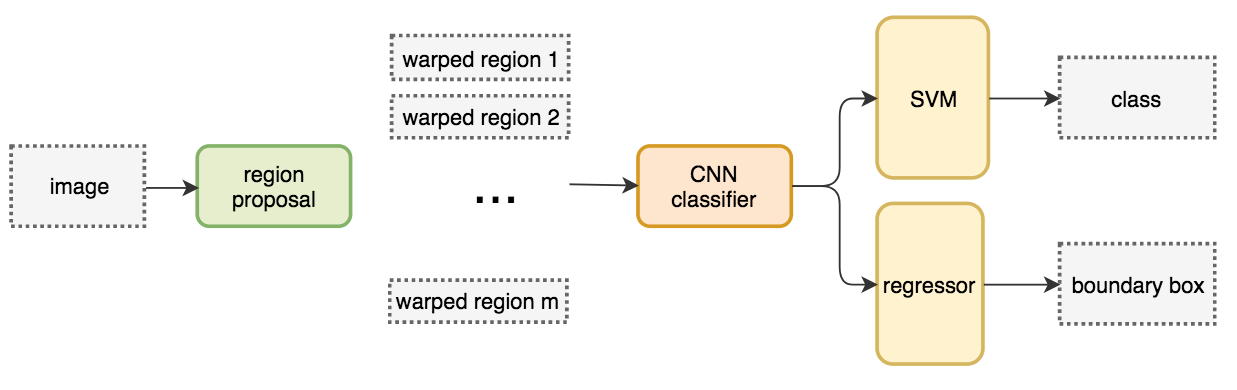
\includegraphics[width=0.8\maxwidth]{../figures/rcnn2.png}
    \caption{Η μέθοδος R-CNN\label{fig:rcnn}}
   \end{center}
\end{figure}


Η ανίχνευση αντικειμένου χρησιμοποιώντας μια μέθοδο παραγωγής προτεινόμενων περιοχών
ενδιαφέροντος και το νευρωνικό δίκτυο R-CNN επιτυγχάνει μικρότερο χρόνο εκτέλεσης
και μεγαλύτερη ακρίβεια σε σχέση με τις μεθόδους κυλιόμενου παραθύρου. Όμως επειδή
κάθε μία από τις 2000 προτεινόμενες περιοχές ενδιαφέροντος επεξεργάζεται ξεχωριστά,
η μέθοδος συνολικά παραμένει αργή τόσο στην εκπαίδευση όσο και στην εξαγωγή αποτελέσματος.
\subsection{Fast R-CNN}\label{sec:fastrcnn}
Το νευρωνικό Fast R-CNN επιλύει το παραπάνω πρόβλημα εφαρμόζοντας τη μέθοδο
εξαγωγής χαρακτηριστικών κατευθείαν πάνω στην αρχική εικόνα. Παράλληλα, με χρήση
μιας μεθόδου παραγωγής προτεινόμενων περιοχών ενδιαφέροντος, εξάγονται οι περιοχές
αυτές οι οποίες συνδυάζονται με το χάρτη χαρακτηριστικών της εικόνας. Το αποτέλεσμα
είναι η παραγωγή των χαρτών χαρακτηριστικών όλων των ROIs σε μόλις δύο βήματα. Οι
χάρτες αυτοί υπόκεινται πρώτα σε μια τεχνική που ονομάζεται ομοιομορφοποίηση
(ROI pooling) για να αποκτήσουν ίσες διαστάσεις και στη συνέχεια δίνονται ως είσοδο
στα πλήρως συνδεδεμένα επίπεδα του νευρωνικού δικτύου για την ταξινόμηση και την
εύρεση του περιγράμματος.


%σχημα
\begin{figure}[htbp]
  \begin{center}
    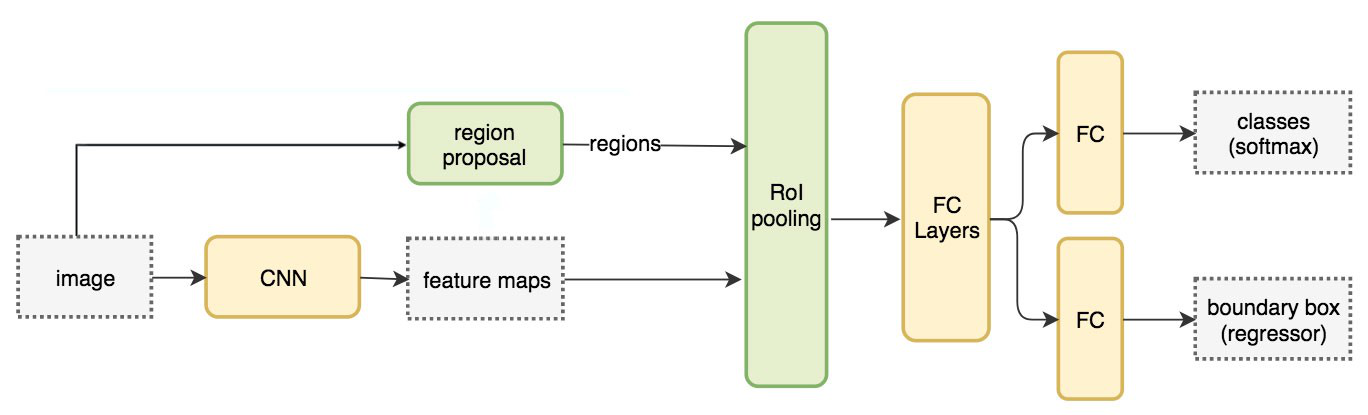
\includegraphics[width=1.1\maxwidth]{../figures/fastrcnn2.png}
    \caption{Η μέθοδος Fast R-CNN\label{fig:fastrcnn}}
   \end{center}
\end{figure}

Το Fast R-CNN ,με τη παραπάνω διαδικασία, αποφεύγει
την εφαρμογή της συνάρτησης εξαγωγής χαρακτηριστικών για κάθε ROI με αποτέλεσμα
ο συνολικός χρόνος εκτέλεσης της μεθόδου για την ανίχνευση του αντικειμένου να
ελαττώνεται σημαντικά.
\subsection{Faster R-CNN}\label{sec:fasterrcnn}
Όπως ήδη έχουμε αναφέρει, η διαδικασία εξαγωγής προτεινόμενων περιοχών ενδιαφέροντος
είναι μια αρκετά ακριβή χρονικά διαδικασία. Πιο συγκεκριμένα, ο συνολικός χρόνος
εκτέλεσης της μεθόδου Fast R-CNN για την εξαγωγή της κλάσης και του περιγράμματος
των αντικειμένων εντός μια εικόνας, διαρκεί κατά μέσο όρο $2,3$ δευτερόλεπτα. Από
αυτό το χρόνο περίπου τα $2$ δευτερόλεπτα χρειάζονται για την εξαγωγή των $2000$
περιοχών ενδιαφέροντος από την αρχική εικόνα.

\begin{figure}[htbp]
  \begin{center}
    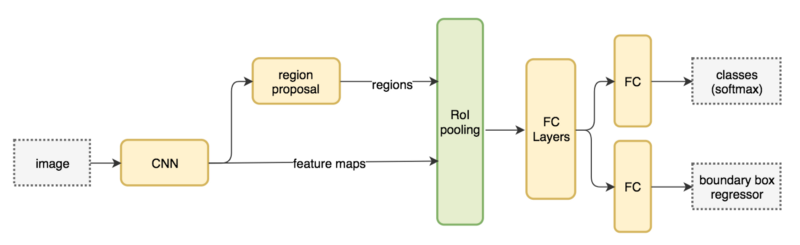
\includegraphics[width=0.9\maxwidth]{../figures/fasterrcnn2.png}
    \caption{Η μέθοδος Faster R-CNN\label{fig:fasterrcnn}}
   \end{center}
\end{figure}

H μέθοδος Faster R-CNN, χρησιμοποιεί την ίδια λογική με τη μέθοδο Fast R-CNN,
αλλά για να βελτιώσει το χρόνο εκτέλεσης της μεθόδου εξαγωγής προτεινόμενων
περιοχών ενδιαφέροντος χρησιμοποιεί εσωτερικά ένα μαθησιακό δίκτυο ώστε οι
περιοχές ενδιαφέροντος να εξάγονται από το χάρτη χαρακτηριστικών της εικόνας. Το
δίκτυο εξαγωγής περιοχών ενδιαφέροντος (Regional Proposal Network - RPN) είναι
πιο αποτελεσματικό και χρειάζεται μόλις $10$ χιλιοστά του δευτερολέπτου για να
δημιουργήσει τα ROIs. Η συνέχεια της μεθόδου είναι όμοια με την παραπάνω \ref{sec:fastrcnn}.
Από το χάρτη χαρακτηριστικών της αρχικής εικόνας και τις προτεινόμενες περιοχές
ενδιαφέροντος σχηματίζονται οι χάρτες χαρακτηριστικών των περιοχών ενδιαφέροντος.
Οι χάρτες αυτοί ,αφού πρώτα υποβληθούν σε ομοιομορφοποίηση (ROI pooling), εισάγονται
στα πλήρως συνδεδεμένα επίπεδα του νευρωνικού δικτύου για την ταξινόμηση του
αντικειμένου και τον προσδιορισμού του περιγράμματος.

\paragraph{Regional Proposal Network - Anchors}\hspace{1pt}\\
\\
Το RPN ,όπως είδαμε, δέχεται ως είσοδο το χάρτη χαρακτηριστικών της εικόνας
και παράγει για κάθε θέση $k$ υποψήφια παράθυρα και $2*k$ τιμές για το οbjectness.
Για παράδειγμα σε ένα χάρτη $8x8$ και για $k=3$ έχουμε:

\begin{figure}[htbp]
  \begin{center}
    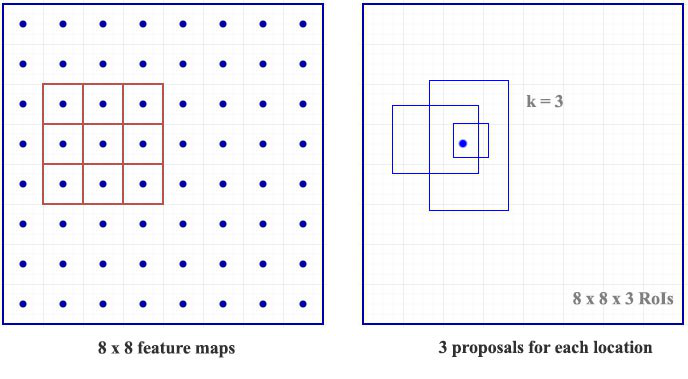
\includegraphics[width=1.4\maxwidth]{../figures/rpn.png}
    \caption{Regional Proposal Network\label{fig:rpn}}
   \end{center}
\end{figure}

Λόγω του ότι τα αντικείμενα έχουν διάφορα σχήματα, θα θέλαμε το προτεινόμενα
παράθυρα να έχουν και αυτά διαφορετικές διαστάσεις. Για το λόγο αυτό λοιπόν οι
προβλέψεις  των παραθύρων δεν υπολογίζονται τυχαία αλλά υπολογίζονται σε σχέση
με κάποια προκαθορισμένα παράθυρα γύρω από κάθε θέση τα οποία ονομάζονται
\textbf{anchors}. Για κάθε λοιπόν προτεινόμενο παράθυρο υπολογίζονται οι διαφορές
$δx$ και $δy$ από την πάνω αριστερή γωνία του αντίστοιχου anchor.

\begin{figure}[htbp]
  \begin{center}
    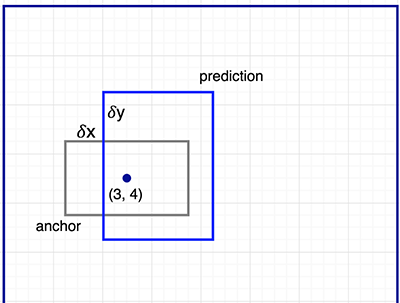
\includegraphics[width=0.4\maxwidth]{../figures/anchor.png}
    \caption{Regional Proposal Network\label{fig:anchor}}
   \end{center}
\end{figure}

Οι anchors προσαρμόζονται ώστε να καλύπτουν τα χαρακτηριστικά αντικειμένων του
πραγματικού κόσμου τόσο σε διαστάσεις, μέγεθος και κλίμακα. Με αυτόν τον τρόπο
η εκπαίδευση του συνολικού δικτύου είναι ελεγχόμενη με την έννοια ότι τα προτεινόμενα
παράθυρα για κάθε θέση είναι ακριβέστερα τόσο στη θέση όσο και στο σχήμα τους.

Σε εφαρμογές πραγματικού περιβάλλοντος ή μέθοδος Faster R-CNN χρησιμοποιεί 9
anchors για κάθε θέση, 3-ων διαφορετικών σχημάτων σε 3 διαφορετικές κλίμακες.

\section{Ανίχνευση αντικειμένων χρησιμοποιώντας ανιχνευτές μονής λήψης}\label{sec:objssd}

Οι ανιχνευτές βασιζόμενοι σε μια περιοχή της εικόνας (Regional Based Detectors)
\ref{sec:objrcnn} είναι αρκετά ακριβείς, όμως ο χρόνος εκτέλεσής τους συνεχίζει
να είναι υψηλός. Π.χ. η μέθοδος Faster R-CNN επεξεργάζεται 7 εικόνες το δευτερόλεπτο
(7 Frames Per Second) από το εκπαιδευτικό σετ PASCAL VOC 2007~\cite{pascal-voc-2007} \flink{http://host.robots.ox.ac.uk/pascal/VOC/}.

\begin{listing}
    \includeminted[text]{../listings/algorcnn.txt}{%
      Regional Proposal Methods}{lst:algorcnn}{linenos}
\end{listing}

Ένας εύκολος τρόπος για να βελτιωθεί ο χρόνος εκτέλεσης της μεθόδου, είναι να
μειωθεί ο χρόνος που χρειάζεται για την επεξεργασία και εξαγωγή αποτελέσματος από
κάθε περιοχή ενδιαφέροντος. Πιο συγκεκριμένα μπορούμε να εξάγουμε την κλάση και το
περίγραμμα ενός αντικειμένου κατευθείαν από το χάρτη χαρακτηριστικών της εικόνας.
Με αυτόν τον τρόπο παρακάμπτουμε τα βήματα παραγωγής και επεξεργασίας των ROIs,
ελαττώνοντας σημαντικά το συνολικό χρόνος εκτέλεσης της μεθόδου.

\begin{listing}
    \includeminted[text]{../listings/algossd.txt}{%
      Single Shot Method}{lst:algossd}{linenos}
\end{listing}

Εξετάζοντας εκ νέου τη μέθοδο κυλιόμενου παραθύρου, παρατηρούμε ότι χρησιμοποιούνται
παράθυρα διαφορετικού σχήματος για διαφορετικούς τύπους αντικειμένων τα οποία
διατρέχουν όλη την εικόνα ή το χάρτη χαρακτηριστικών της. Το βασικό μειονέκτημα
αυτής της μεθόδου είναι ότι το παράθυρο το οποίο διατρέχει την εικόνα χρησιμοποιείται
από τη μέθοδο ως το τελικό περίγραμμα του εντοπιζόμενου αντικειμένου. Επομένως
η μέθοδος χρησιμοποιεί όλα τα πιθανά μεγέθη και σχήματα παραθύρου για να μπορεί
να εντοπίσει τα αντικείμενα όλων των διαφορετικών τύπων και μεγεθών.
\paragraph{} \hspace{0em} \\
Ένας πιο αποτελεσματικός τρόπος, είναι να θεωρήσουμε το παράθυρο αυτό
όχι το τελικό περίγραμμα του αντικειμένου, αλλά μια αρχική πρόβλεψη για τη θέση του.
Επομένως, στη συνέχεια θα χρειαστούμε έναν ανιχνευτή για τον \texttt{ταυτόχρονο}
προσδιορισμό της κλάσης και του πραγματικού περιγράμματος του αντικειμένου.

Ο τρόπος αυτός μοιάζει αρκετά με τη λειτουργία των anchors που χρησιμοποιεί για να
εξάγει τις περιοχές ενδιαφέροντος το Regional Proposal Network στη μέθοδο Faster R-CNN
\ref{fig:anchor}. Αντιθέτως όμως, ένας ανιχνευτής μονής λήψης προβλέπει τόσο
το περίγραμμα (boundary box), όσο και την κλάση του αντικειμένου την ίδια χρονική
στιγμή.

Η διαφορά έγκειται στο γεγονός ότι το Faster R-CNN χρησιμοποιεί ένα συνελικτικό
φίλτρο για να κάνει μια πρόβλεψη 5 παραμέτρων για κάθε θέση στο χάρτη χαρακτηριστικών.
Οι 4 από αυτές αναφέρονται στο προβλεπόμενο bounding box από το τρέχον anchor ενώ η
άλλη μας δίνει το ποσοστό αντικειμενικότητας του anchor. Επομένως επαναφέροντας το
παράδειγμα της προηγούμενης ενότητας \ref{sec:fasterrcnn}, εφαρμόζοντας ένα συνελικτικό φίλτρο
διαστάσεων $3 \times 3 \times D \times 5$ σε ένα χάρτη χαρακτηριστικών
$8 \times 8 \times D$ εκείνος τελικά μετατρέπεται σε ένα χάρτη διαστάσεων $8 \times 8 \times 5$.

Ένας ανιχνευτής μονής λήψης (Single Shot) κάνει επιπλέον $C$ προβλέψεις για την
κλάση του αντικειμένου για κάθε θέση του χάρτη χαρακτηριστικών. Με αυτόν τον τρόπο
για $C = 20$ το συνελικτικό φίλτρο που χρησιμοποιείται έχει διαστάσεις
$ 3 \times 3 \times 25(5 + C)$ και μετατρέπει τον χάρτη χαρακτηριστικών από $8 \times 8 \times D$
σε $8 \times 8 \times 25$.

Γενικά, οι ανιχνευτές μονής λήψης πετυχαίνουν αρκετά καλύτερους χρόνους εκτέλεσης
υστερώντας όμως σε ακρίβεια σε σχέση με τις μεθόδους που χρησιμοποιούν περιοχές ενδιαφέροντος.
Επιπλέον έχει παρατηρηθεί ότι δυσκολεύονται να ανιχνεύσουν αντικείμενα που βρίσκονται
πολύ κοντά ή είναι πολύ μικρά.

\subsection{Single Shot Multibox Detector (SSD)}\label{sec:ssd}

Ο ανιχνευτής SSD~\cite{liu2016ssd} σχεδιάστηκε για την ανίχνευση αντικειμένων σε πραγματικό χρόνο.
Η τυπική του υλοποίηση χρησιμοποιεί το νευρωνικό δίκτυο \textbf{VGG16}
~\cite{DBLP:journals/corr/SimonyanZ14a} για την εξαγωγή χαρακτηριστικών
από μια εικόνα. Το αποτέλεσμα προωθείται σε μια αλληλουχία συνελικτικών επιπέδων
για να καταλήξει τελικά σε συνελικτικά φίλτρα τα οποία πραγματοποιούν και την
τελική πρόβλεψη.

\begin{figure}[htbp]
  \begin{center}
    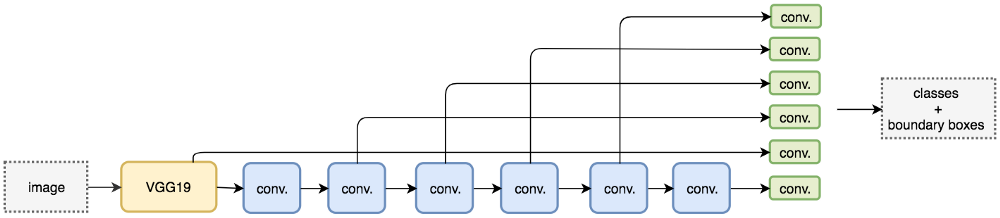
\includegraphics[width=0.9\maxwidth]{../figures/ssd.png}
    \caption{Η μέθοδος Single Shot Multibox Detector\label{fig:ssd}}
   \end{center}
\end{figure}

Για κάθε θέση του χάρτη χαρακτηριστικών το SSD πραγματοποιεί $4$ προβλέψεις. Κάθε
πρόβλεψη αποτελείται από ένα περίγραμμα (τεσσάρων παραμέτρων) και $21$  βαθμολογίες·
μία για κάθε κλάση, όπως αυτές προσδιορίστηκαν από το διαγωνισμό PASCAL VOC~\cite{pascal-voc-2007}.
Από αυτές κρατάει την υψηλότερη ως την προβλεπόμενη κλάση του αντικειμένου.


\subsection{Η μέθοδος You Only Look Once (YOLO)}\label{sec:yolo}

Το YOLO είναι ένας ανιχνευτής μονής λήψης. Χρησιμοποιεί το νευρωνικό δίκτυο
DarkNet~\cite{darknet13} για την εξαγωγή των χαρακτηριστικών, ακολουθούμενο από
συνελικτικά επίπεδα. Σε αντίθεση με τη μέθοδο SSD, δεν χρησιμοποιεί τους χάρτες
χαρακτηριστικών με διαφορετικές διαστάσεις από κάθε επίπεδο για να κάνει προβλέψεις,
αλλά αντί αυτού ανασχηματίζει και συνθέτει διάφορους χάρτες πραγματοποιώντας από
αυτούς τις προβλέψεις. Για παράδειγμα ανασχηματίζει ένα επίπεδο $28 \times 28 \times 512$
σε ένα $14 \times 14 \times 2048$. Στη συνέχεια παίρνει τον παραγόμενο από αυτό το
επίπεδο χάρτη χαρακτηριστικών και τον συνθέτει με ένα μικρότερης ανάλυσης χάρτη
$14 \times 14 \times 1024$. Στη συνέχεια εφαρμόζει στο νέο αυτό χάρτη διαστάσεων
$14 \time 14 \times 3072$ συνελικτικά φίλτρα για να πραγματοποιήσει στη συνέχεια
τις προβλέψεις.

Το YOLOv2~\cite{7780460} πετυχαίνει $63.4$ μέση ακρίβεια (mean Average Precision - mAP).
Με διάφορες βελτιώσεις το YOLOv2~\cite{DBLP:journals/corr/RedmonF16} καταφέρνει να αυξήσει την mAP σε 78.6 ενώ το
YOLO900~\cite{DBLP:journals/corr/RedmonF16} καταφέρνει να ανιχνεύσει έως και 9000 διαφορετικές κατηγορίες αντικειμένων.


%σχηματα + πινακες

\section{Άλλες μέθοδοι για την ανίχνευση αντικειμένων}\label{sec:objmethods}


\subsection{Πλήρως Συνελικτικά Δίκτυα βασιζόμενα σε μια περιοχή της εικόνας
(Region-based Fully Convolutional Networks - \\R-FCN~\cite{DBLP:journals/corr/DaiLHS16})}\label{sec:rfcn}

Στο σχήμα ~\ref{lst:algorcnn} είδαμε τη γενική μέθοδο που χρησιμοποιούν οι
τεχνικές συνελικτικών νευρωνικών δικτύων. Οι τεχνικές αυτές στο βήμα 5, όπου
πραγματοποιείται η ανίχνευση, επεξεργάζονται τους χάρτες χαρακτηριστικών των
ROIs και παράγουν αποτελέσματα μέσω πλήρως συνδεδεμένων επιπέδων. Η επεξεργασία
δεδομένων από πλήρως συνδεδεμένα επίπεδα είναι μια σχετικά ακριβή διαδικασία και
αν σκεφτούμε ότι στην προκείμενη περίπτωση το νευρωνικό επεξεργάζεται 2.000 ROIs,
τότε η συνολική διαδικασία είναι αρκετά ακριβή.

%σχήμα
\begin{figure}[htbp]
  \begin{center}
    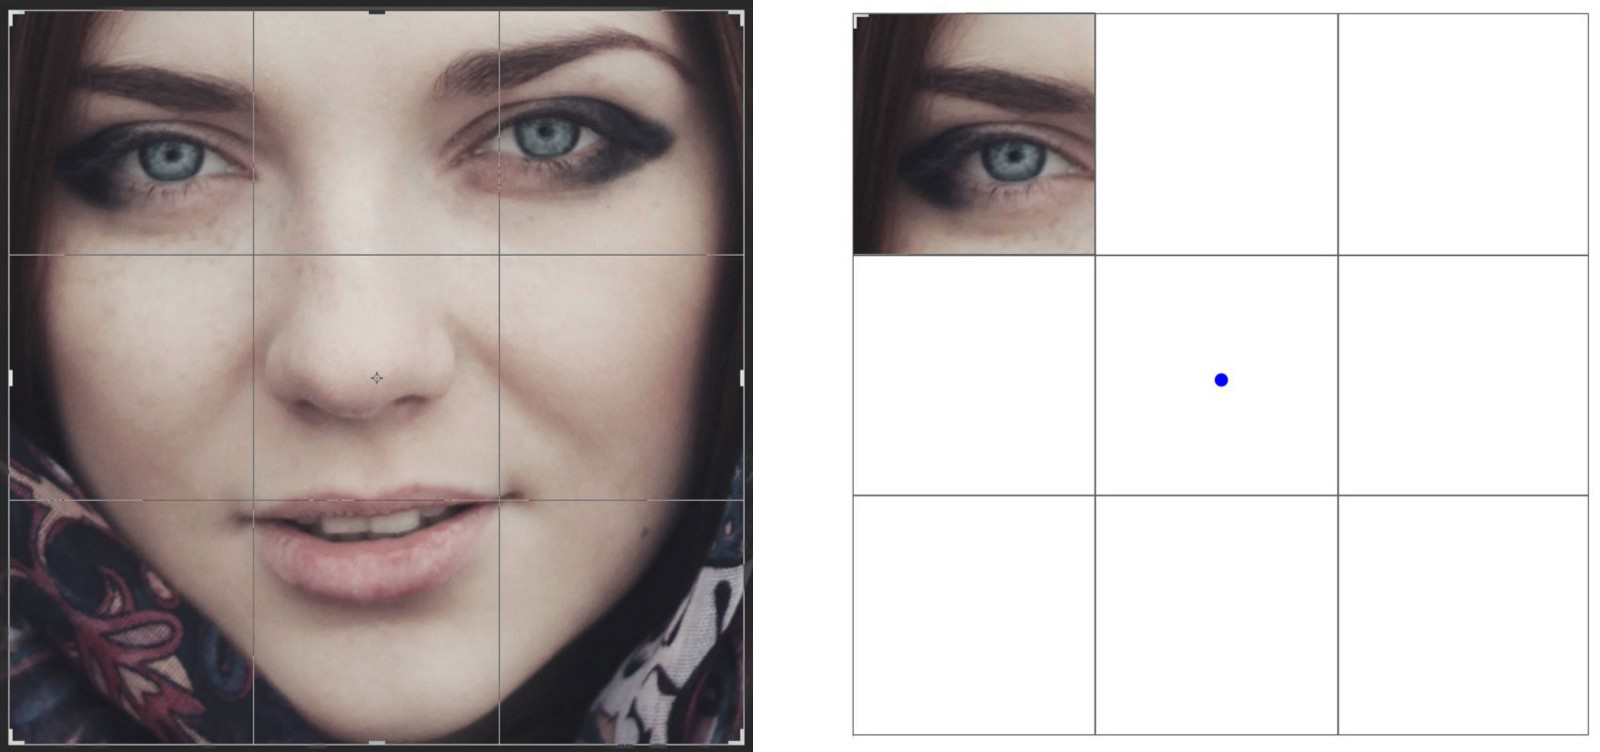
\includegraphics[width=0.8\maxwidth]{../figures/rfcn.png}
    \caption{H τεχνική R-FCN\label{fig:fpn}}
   \end{center}
\end{figure}

Αν λοιπόν μειωθεί ο χρόνος επεξεργασίας που χρειάζεται για κάθε ROI τότε θα
βελτιωθεί και η ταχύτητα εκτέλεσης του ανιχνευτή. Η τεχνική R-FCN εκμεταλλεύεται
τους χάρτες χαρακτηριστικών κάποιων υποπεριοχών του αντικειμένου και της θέσης του
για να εξάγει ένα τελικό συμπέρασμα για την κλάση και τη θέση του αντικειμένου. Ένα
απλοϊκό παράδειγμα έχει να κάνει με την ανίχνευση προσώπου. Σε κάθε υποψήφιο ROI
ελέγχεται αν συγκεκριμένες υποπεριοχές του πληρούν τις προϋποθέσεις ενός προσώπου.
Π.χ. το δεξί μάτι να είναι στην πάνω αριστερή γωνία, το αριστερό στην πάνω δεξιά κ.ο.κ.
Με αυτό τον τρόπο συνδυάζοντας τις επιμέρους  βαθμολογίες για κάθε υποπεριοχή ενός
ROI το δίκτυο εξάγει γρηγορότερα αποτελέσματα χωρίς απώλειες σε ακρίβεια.

\subsection{Δίκτυα Πυραμίδας Χαρακτηριστικών (Feature Pyramid Networks FPN~\cite{DBLP:journals/corr/LinDGHHB16})}\label{sec:fpn}
Τα δίκτυα πυραμίδας δεν αποτελούν από μόνα τους ένα ανιχνευτή αντικειμένων, αλλά
ενσωματώνονται στις υπάρχουσες τεχνικές για την ανίχνευση αντικειμένων σε διάφορες
κλίμακες (μεγέθη). Τα Δίκτυα Πυραμίδας παράγουν πυραμίδες χαρτών χαρακτηριστικών από
μια εικόνα οι οποίοι βελτιώνουν την ταχύτητα και την ακρίβεια του τελικού αποτελέσματος.
Στο παρακάτω σχήμα \ref{fig:fpn} τα $P2, P3, P4, P5$ είναι αναπαριστούν την προαναφερθείσα πυραμίδα.

%σχήμα
\begin{figure}[htbp]
  \begin{center}
    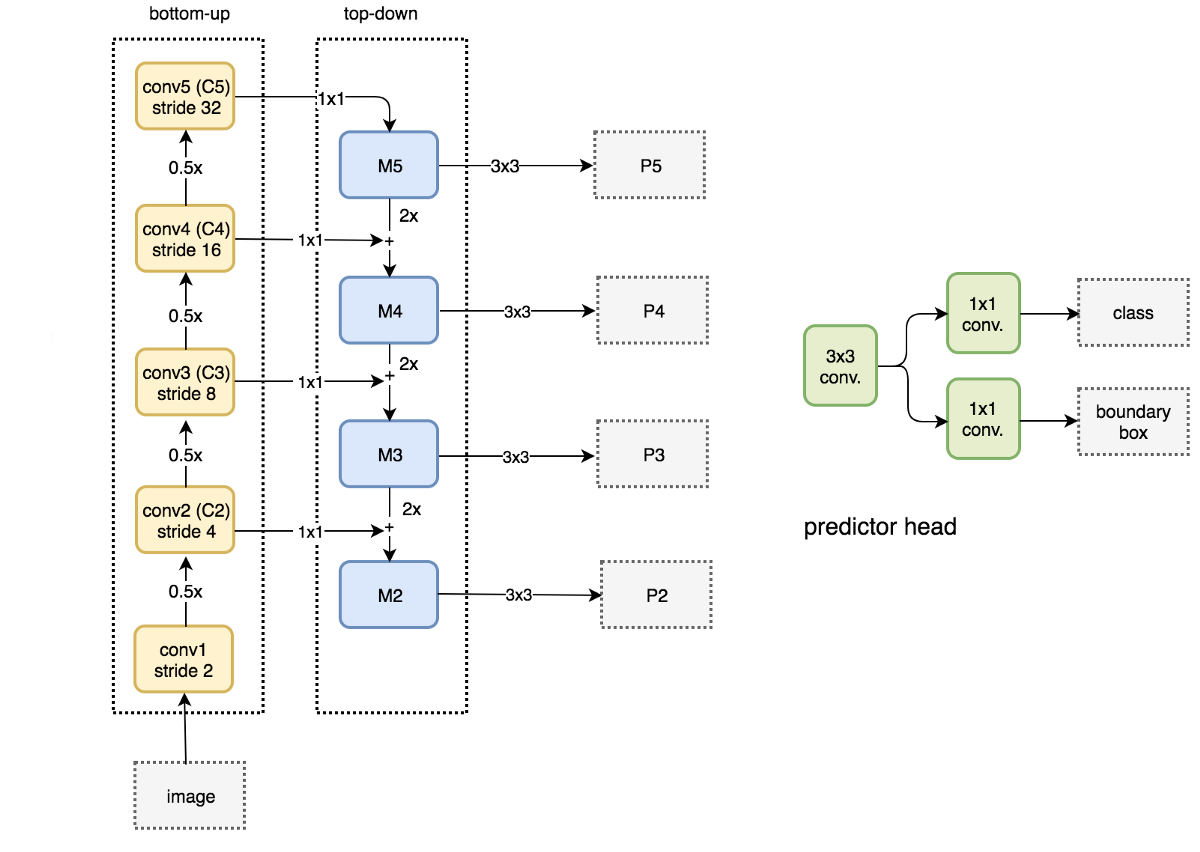
\includegraphics[width=0.8\maxwidth]{../figures/fpn.png}
    \caption{Το FPN του σχήματος τροφοδοτεί έναν Object Detector\label{fig:fpn}}
   \end{center}
\end{figure}

Υπάρχουν 2 πυραμιδικές διαδρομές από χάρτες, μία από κάτω προς τα πάνω και μία
από πάνω προς τα κάτω. Τα χαμηλότερα επίπεδα χαρτών έχουν υψηλότερη ανάλυση αλλά
μικρότερη πυκνότητα πληροφορίας σε σχέση με τα ανώτερα. Στο SSD~\ref{sec:ssd} για παράδειγμα
χρησιμοποιούνται μόνο τα ανώτερα επίπεδα (πλούσια σε πληροφορία) για τον εντοπισμό
της θέσης ενός αντικειμένου. Παρόλο που η πρόβλεψη είναι ακριβέστερη και πιο γρήγορη,
λόγω της μικρότερης ανάλυσης το SSD δυσκολεύεται να ανιχνεύσει μικρά αντικείμενα.
Ένα FPN ανακατασκευάζει από τα ανώτερα επίπεδα χαρτών, νέα επίπεδα με περισσότερες διαστάσεις.
Μάλιστα επειδή τα νέα  αυτά επίπεδα υστερούν σε ακρίβεια -λόγω του ότι προέρχονται ύστερα από υποδειγματοληψία
και υπερδειγματοληψία του αρχικού χάρτη- είναι συνδεδεμένα με τους χάρτες χαρακτηριστικών
ιδίων διαστάσεων. Με αυτόν τον τρόπο ο ανιχνευτής υποψήφιων θέσεων αντικειμένων
λειτουργεί καλύτερα.
\paragraph{} \hspace{0em} \\
Ένα FPN είπαμε είναι ένα εξαγωγέας χαρακτηριστικών από μια εικόνα. Στις διάφορες
μεθόδους ακολουθείται κυρίως από ένα RPN \ref{sec:fasterrcnn} το οποίο εξάγει τα ROIs.
Ανάλογα με το μέγεθος του κάθε ROI επιλέγεται ο χάρτης χαρακτηριστικών κατάλληλων
διαστάσεων για να εξαχθούν οι υποπεριοχές χαρακτηριστικών. Στη συνέχεια κατά τα
γνωστά κατά τα άλλα οι υποπεριοχές αυτές υπόκεινται σε ομαλοποίηση (ROI pooling)
για να επεξεργαστούν στη συνέχεια από πλήρως συνδεδεμένα επίπεδα και να εξαχθεί
η κλάση και το περίγραμμα του αντικειμένου.


\section{Συνολική αποτίμηση}\label{sec:objdetchoice}

Στο κεφάλαιο αυτό έγινε μια καταγραφή των σύγχρονων τεχνικών ανίχνευσης αντικειμένων
χρησιμοποιώντας νευρωνικά δίκτυα. Είδαμε την εξέλιξη των μεθόδων που βασίζονται
σε προτεινόμενες περιοχές ενδιαφέροντος καταλήγοντας στην πλέον σύγχρονη Faster R-CNN
\ref{sec:fasterrcnn}. Αναλύσαμε επιπλέον την τεχνική των ανιχνευτών μονής λήψης
και είδαμε ορισμένες σύγχρονες μεθόδους όπως η SSD \ref{sec:ssd} και η YOLO \ref{sec:yolo}.
Κάθε μια μέθοδος έχει τα δικά της χαρακτηριστικά (mAP, χρόνο εκτέλεσης, κατανάλωση μνήμης)
ανάλογα με το περιβάλλον που χρησιμοποιείται. Για παράδειγμα είδαμε ότι η μέθοδος
SSD αναγνωρίζει σχετικά μεγάλα αντικείμενα με μεγάλη ακρίβεια ενώ έχει αρκετά
μικρότερη ακρίβεια σε μικρά.

Στα πλαίσια της παρούσας εργασίας έγινε ανάλυση των χαρακτηριστικών της κάθε μεθόδου
και αυστηρός προσδιορισμός των απαιτήσεων του υλοποιηθέντος συστήματος για την
επιλογή της κατάλληλης μεθόδου. Η μέθοδος η οποία χρησιμοποιήθηκε για την
ανίχνευση αντικειμένων ήταν η SSD χρησιμοποιώντας το νευρωνικό δίκτυο MobileNet~\cite{DBLP:journals/corr/HowardZCKWWAA17}
για την εξαγωγή των χαρακτηριστικών από την εικόνα.

\begin{figure}[htp]
    \centering
    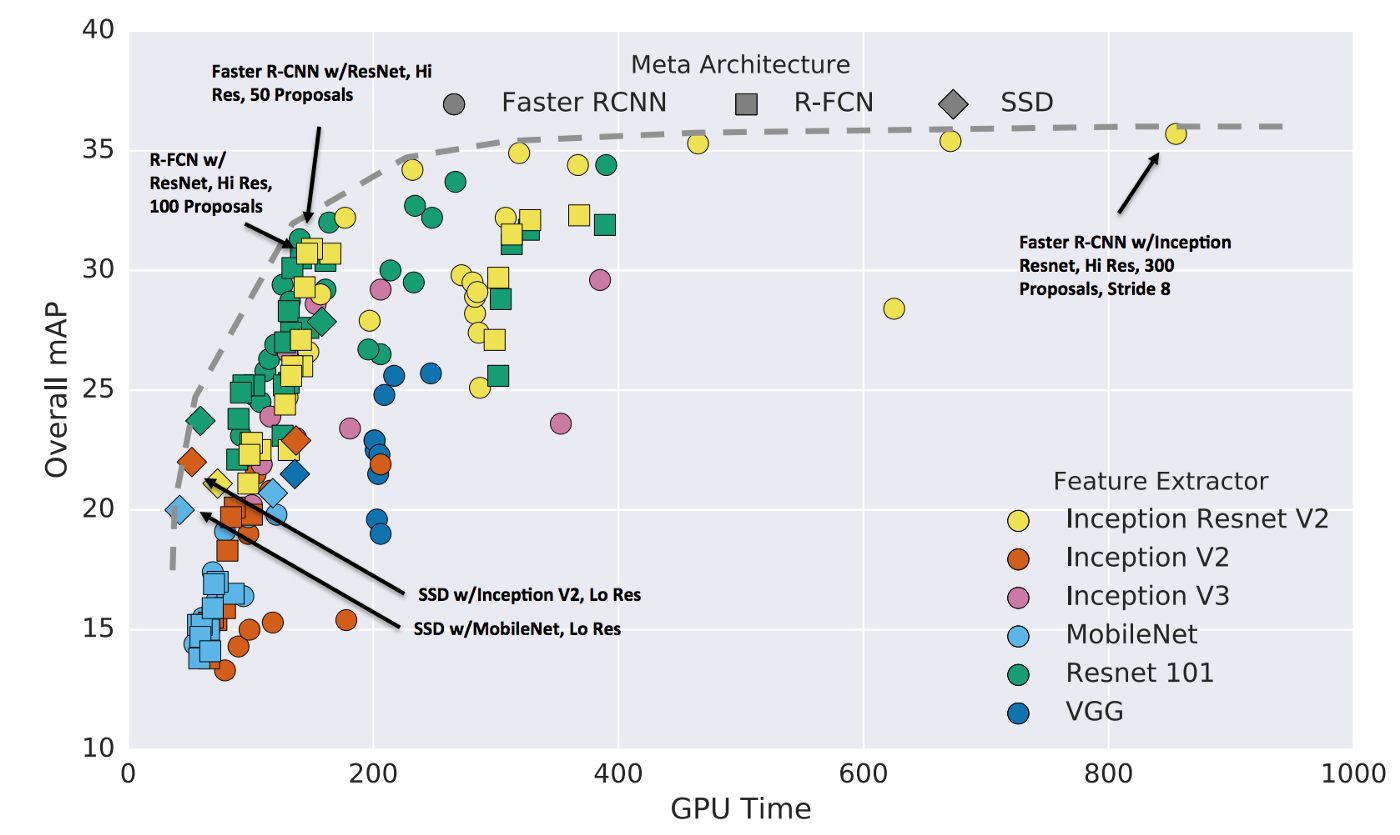
\includegraphics[width=.50\maxwidth]{../figures/speedvsaccuracy.png}\hfill
    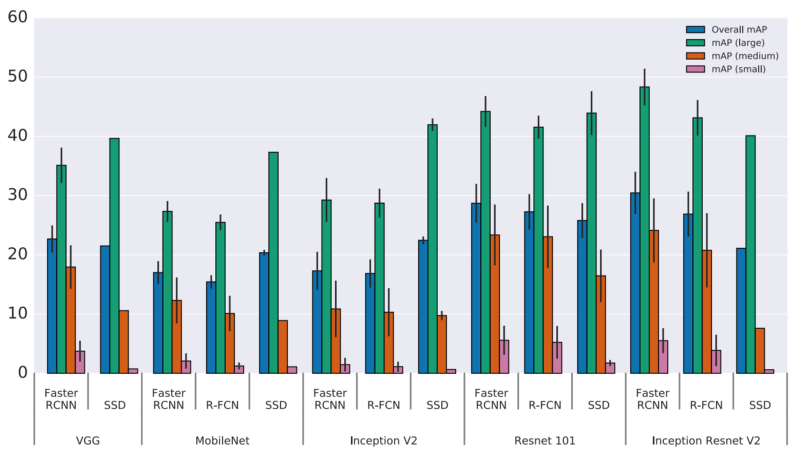
\includegraphics[width=.50\maxwidth]{../figures/imagesize.png}\hfill
    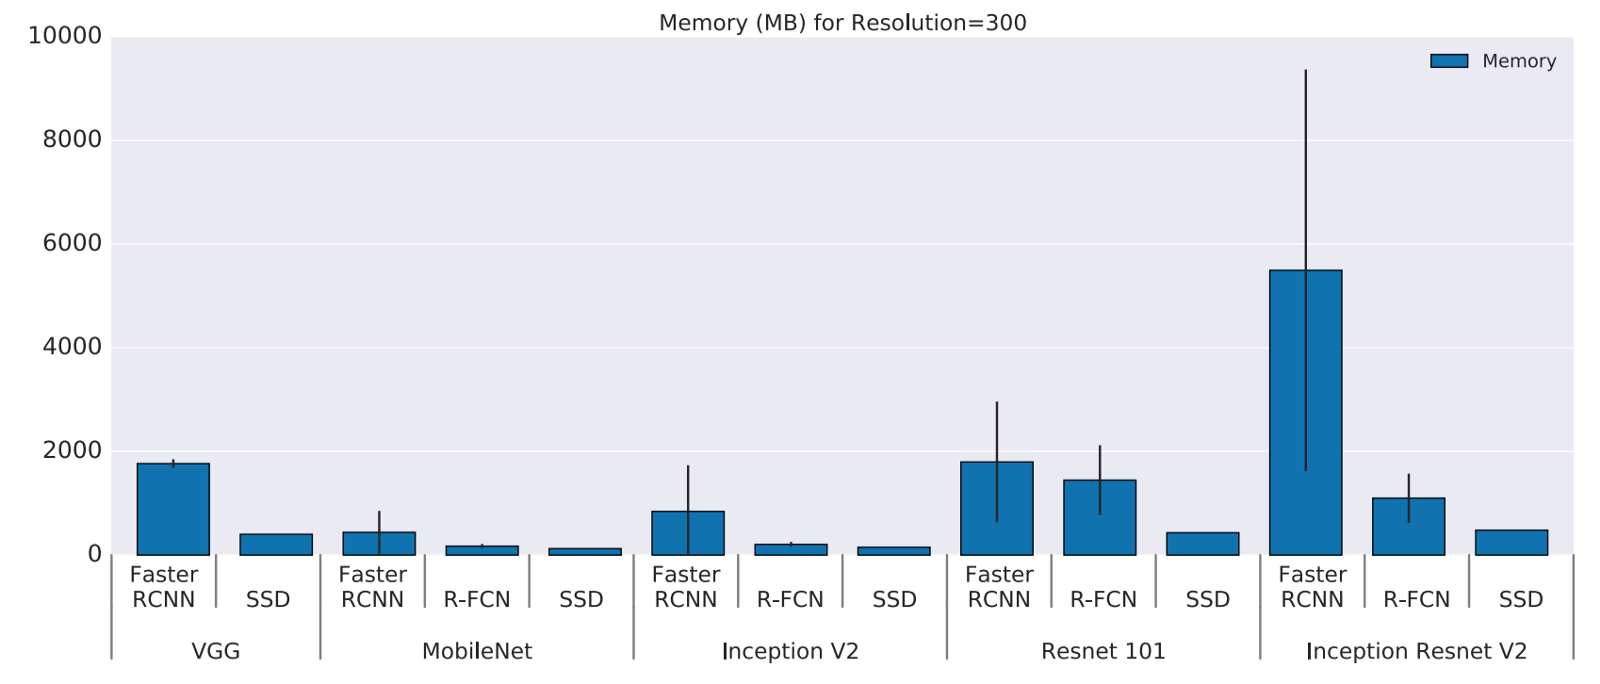
\includegraphics[width=.52\maxwidth]{../figures/memory.png}\hfill

    \caption{α) Χρόνος εκτέλεσης κ mAP β) Μέγεθος αντικειμένου γ) Μνήμη}
    \label{fig:bee}

\end{figure}

Τα παραπάνω αποτελέσματα ελήφθησαν χρησιμοποιώντας το σύνολο εικόνων MS COCO.

Ο βασικός λόγος που επιλέχθηκε η συγκεκριμένη μέθοδος ήταν η απαίτηση του συστήματός μας
για μικρό χρόνος εκτέλεσης καθώς και ο περιορισμός του σε μνήμη. Πιο συγκεκριμένα,
λόγω του ότι το σύστημα επεξεργάζεται βίντεο δηλαδή μια αλληλουχία εικόνων και μάλιστα
κινηματογραφικού επιπέδου, σημαίνει ότι ο συνολικός αριθμός των frames που εισάγεται
σε κάθε κύκλο επεξεργασίας είναι αρκετά μεγάλος. Για να επιτύχουμε ένα χρόνο επεξεργασίας
που θα είναι ανταγωνιστικός χρειάζεται να επενδύσουμε σε μια γρήγορη μέθοδοι. Επίσης
σε ένα βίντεο στο πραγματικό κόσμο υπάρχουν αρκετές εκατοντάδες αντικείμενα τα οποία
όμως δεν εμπίπτουν όλα στο ενδιαφέρον του χρήστη. Για το χρήστη τα σημαντικά αντικείμενα
είναι εκείνα που με κάποιο τρόπο προσδιορίζουν το γενικότερο θέμα του βίντεο. Για παράδειγμα
ένα ντοκιμαντέρ για τα ζώα, προβάλλει πολλά είδη ζώων ένα σχετικά μεγάλο αντικείμενο. Το
SSD δεν έχει πρόβλημα να αναγνωρίσει αντικείμενα τέτοιου μεγέθους, οπότε για τις
συγκεκριμένες ανάγκες του συστήματός μας οι προβλέψεις του ήταν ανταγωνιστικές. Τέλος
το γεγονός της περιορισμένης μνήμης των μηχανημάτων που διαθέταμε μας οδήγησε περισσότερο
στην επιλογή του δικτύου MobileNet για την εξαγωγή των χαρακτηριστικών το οποίο
σχεδιάστηκε με στόχο να έχει μικρές απαιτήσεις σε μνήμη και υπολογιστική ισχύ ώστε
να κάνει τις μεθόδους ανίχνευσης αντικειμένου υλοποιήσιμες σε έξυπνες συσκευές κινητής
τηλεφωνίας.
